\subsection{Tenant types}
\label{sec:application:building_the_model:tenant_types}

In the twelfth step, a field referencing the new enumeration type is introduced. \cref{subsec:library_of_transformations:type_level_transformations:enum_fields} is used to introduce the enumeration field on the type level, while on the instance level, \cref{subsec:library_of_transformations:instance_level_transformations:enum_field_values} is used to introduce the values.

The $classtype$ of the new field is $.\type{Tenant}$, as the field will be defined for tenants. The $name$ of the new field is $\type{type}$ and the $enumid$ is $.\type{TenantType}$. Furthermore, the set of $enumvalues$ is equal to the set of values for the $.\type{TenantType}$ enumeration type, so $enumvalues = \{\type{REGULAR}, \type{SUBTENANT}\}$. Then, $enumids$ returns for each enumeration value the corresponding node identifier used in the GROOVE graph, while $enumob$ lists the corresponding internal node id.

The set of objects of which the value is set is equal to all tenant objects, so $objects = \{Tenant1, Tenant2,$\\$ Tenant3, Tenant4, Tenant5\}$. The $values$ function is defined as follows:
\begin{align*}
    values = values = \{&(Tenant1, \type{REGULAR}), (Tenant2, \type{REGULAR}), (Tenant3, \type{REGULAR}), \\&(Tenant4, \type{REGULAR}), (Tenant5, \type{SUBTENANT})\}
\end{align*}

The following model is obtained:

\LTXtable{\textwidth}{tex/06_application/02_building_the_model/tables/12_tenant_types.tex}

\begin{figure}[p]
    \centering
    \begin{subfigure}{0.98\textwidth}
        \centering
        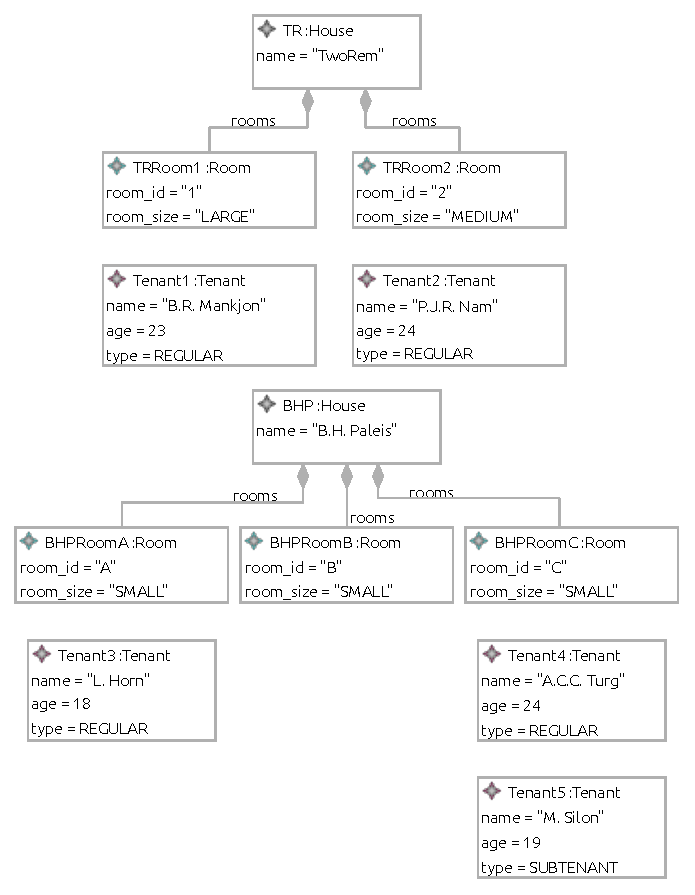
\includegraphics{images/06_application/instance_model/step12.pdf}
        \caption{Instance Model $Im_{12}$}
        \label{fig:application:building_the_model:tenant_types:ecore:instance_model}
    \end{subfigure}
    \\
    \begin{subfigure}{0.98\textwidth}
        \centering
        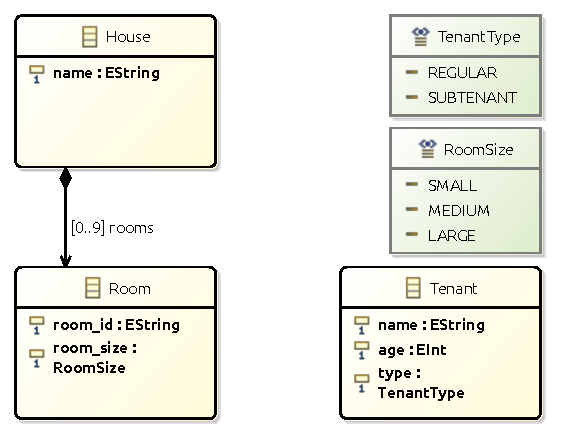
\includegraphics{images/06_application/type_model/step12.pdf}
        \caption{Type Model $Tm_{12}$}
        \label{fig:application:building_the_model:tenant_types:ecore:type_model}
    \end{subfigure}
    \caption{The Ecore model after step 12}
    \label{fig:application:building_the_model:tenant_types:ecore}
\end{figure}

\begin{figure}[p]
    \centering
    \begin{subfigure}{0.98\textwidth}
        \centering
        % To use this figure in your LaTeX document
% import the package groove/resources/groove2tikz.sty
%
\begin{tikzpicture}[scale=\tikzscale,name prefix=step12-]
\node[type_node] (n0) at (0.740, -0.400) {\ml{\textbf{House}\\name: \textbf{string}}};
\node[type_node] (n1) at (0.730, -1.585) {\ml{\textbf{Room}\\room\_id: \textbf{string}}};
\node[type_node] (n2) at (2.380, -0.560) {\ml{\textbf{RoomSize}\\\textit{LARGE}\\\textit{MEDIUM}\\\textit{SMALL}}};
\node[type_node] (n3) at (2.500, -1.590) {\ml{\textbf{Tenant}\\age: \textbf{int}\\name: \textbf{string}}};
\node[abstract_node] (n4) at (4.710, -0.980) {\ml{\textit{\textbf{TenantType}}}};
\node[type_node] (n5) at (3.810, -0.320) {\ml{\textbf{TenantType\$REGULAR}}};
\node[type_node] (n6) at (5.680, -0.320) {\ml{\textbf{TenantType\$SUBTENANT}}};

\path[basic_edge, composite](n0.south -| 0.730, -1.585) -- node[lab] {\ml{rooms}} (n1) ;
\path[basic_edge] (n1)  -- node[lab] {\ml{room\_size}} (n2) ;
\path[basic_edge] (n3)  -- node[lab] {\ml{type}} (n4) ;
\path[subtype_edge] (n5)  --  (n4) ;
\path[subtype_edge] (n6)  --  (n4) ;
\end{tikzpicture}

        \caption{Instance Graph $IG_{12}$}
        \label{fig:application:building_the_model:tenant_types:groove:instance_graph}
    \end{subfigure}
    \\
    \begin{subfigure}{0.98\textwidth}
        \centering
        % To use this figure in your LaTeX document
% import the package groove/resources/groove2tikz.sty
%
\begin{tikzpicture}[scale=\tikzscale,name prefix=step12-]
\node[type_node] (n0) at (0.740, -0.400) {\ml{\textbf{House}\\name: \textbf{string}}};
\node[type_node] (n1) at (0.730, -1.585) {\ml{\textbf{Room}\\room\_id: \textbf{string}}};
\node[type_node] (n2) at (2.380, -0.560) {\ml{\textbf{RoomSize}\\\textit{LARGE}\\\textit{MEDIUM}\\\textit{SMALL}}};
\node[type_node] (n3) at (2.500, -1.590) {\ml{\textbf{Tenant}\\age: \textbf{int}\\name: \textbf{string}}};
\node[abstract_node] (n4) at (4.710, -0.980) {\ml{\textit{\textbf{TenantType}}}};
\node[type_node] (n5) at (3.810, -0.320) {\ml{\textbf{TenantType\$REGULAR}}};
\node[type_node] (n6) at (5.680, -0.320) {\ml{\textbf{TenantType\$SUBTENANT}}};

\path[basic_edge, composite](n0.south -| 0.730, -1.585) -- node[lab] {\ml{rooms}} (n1) ;
\path[basic_edge] (n1)  -- node[lab] {\ml{room\_size}} (n2) ;
\path[basic_edge] (n3)  -- node[lab] {\ml{type}} (n4) ;
\path[subtype_edge] (n5)  --  (n4) ;
\path[subtype_edge] (n6)  --  (n4) ;
\end{tikzpicture}

        \caption{Type Graph $TG_{12}$}
        \label{fig:application:building_the_model:tenant_types:groove:type_graph}
    \end{subfigure}
    \caption{The GROOVE graphs after step 12}
    \label{fig:application:building_the_model:tenant_types:groove}
\end{figure}

A visual representation of $Tm_{12}$ and $Im_{12}$ can be found in \cref{fig:application:building_the_model:tenant_types:ecore}. Similarly, a visual representation of $TG_{12}$ and $IG_{12}$ can be found in \cref{fig:application:building_the_model:tenant_types:groove}. Please note that because of the definitions of $f_{12}(Im_{12})$ and $f'_{12}(IG_{12})$, we have that $f_{12}(Im_{12}) = IG_{12}$ and $f'_{12}(IG_{12}) = Im_{12}$. Furthermore, $f_{12}(Im_{12})$ and $f'_{12}(IG_{12})$ are valid mapping functions themselves, such that they can be combined with another mapping function in the next step.

The previous step showed how two different encodings of an enumeration type were combined within the same model. This step concludes the combination of these encodings by showing that it is possible to reference values from the tenant type enumeration type, even though it is encoded in a different encoding than the room sizes enumeration type.

\afterpage{\FloatBarrier}